% pdflatex project_proposal.tex && bibtex project_proposal.aux && pdflatex project_proposal.tex && open project_proposal.pdf
\documentclass[a4paper,pagesize 10pt]{scrartcl}

\usepackage{graphicx}
%\usepackage{scalefnt}
%\usepackage{textfit}
\usepackage[square,sort,comma,numbers]{natbib}
\usepackage{url}

\begin{document}


\begin{center}{\Huge\textbf{Project Proposal}}\end{center}
\begin{center}{\Large\textbf{Body Animation}}\end{center}

\section{Abstract}

%
%Write a short abstract of your planned project.
%
%Cite papers that you want to use as references (e.g. Adelson et al.~\cite{adelson1984pyramid}).
%
%Include an overview figure that shows your planned processing pipeline.
%


\begin{flushleft}
The goal of this project is to implement the famous German game “Torwandschießen”, where the player has to kick a football through circular openings on an erected goal post with a limited number of tries. This team which has the most successful shots wins.
\end{flushleft}

\begin{flushleft}
We plan to build this using a kinect and its skeleton tracking SDK \cite{kinect_basic} to map a player and his movements to a rigged 3d avatar. The program will detect the motion in which the player kicks, which then calculates the force and applies it to a virtual ball that is projected to a virtual “Torwand”.
\end{flushleft}

\begin{flushleft}
We plan to simulate the virtual ball and the “Torwand” in AR/MR using Microsoft Holo-lens \cite{hololens}. The Holo-lens would run a Unity application where we use the motion of the player tracked from the Kinect to simulate the forces acting on the virtual ball in order to project it, which can be achieved using the Unity physics engine \cite{unity}.
\end{flushleft}

\begin{flushleft}
From the player’s perspective, he wears the Holo-lens standing in front of a kinect sensor. He sees the virtual ball and the “Torwand” through the Holo-lens, he simply kicks the virtual ball towards the “Torwand”.
\end{flushleft}

\begin{flushleft}
This works is going to be based on multiple papers, see References \cite{source1} \cite{source2} \cite{source3} \cite{source4} 
\end{flushleft}

\begin{figure}[h]
	\centering
	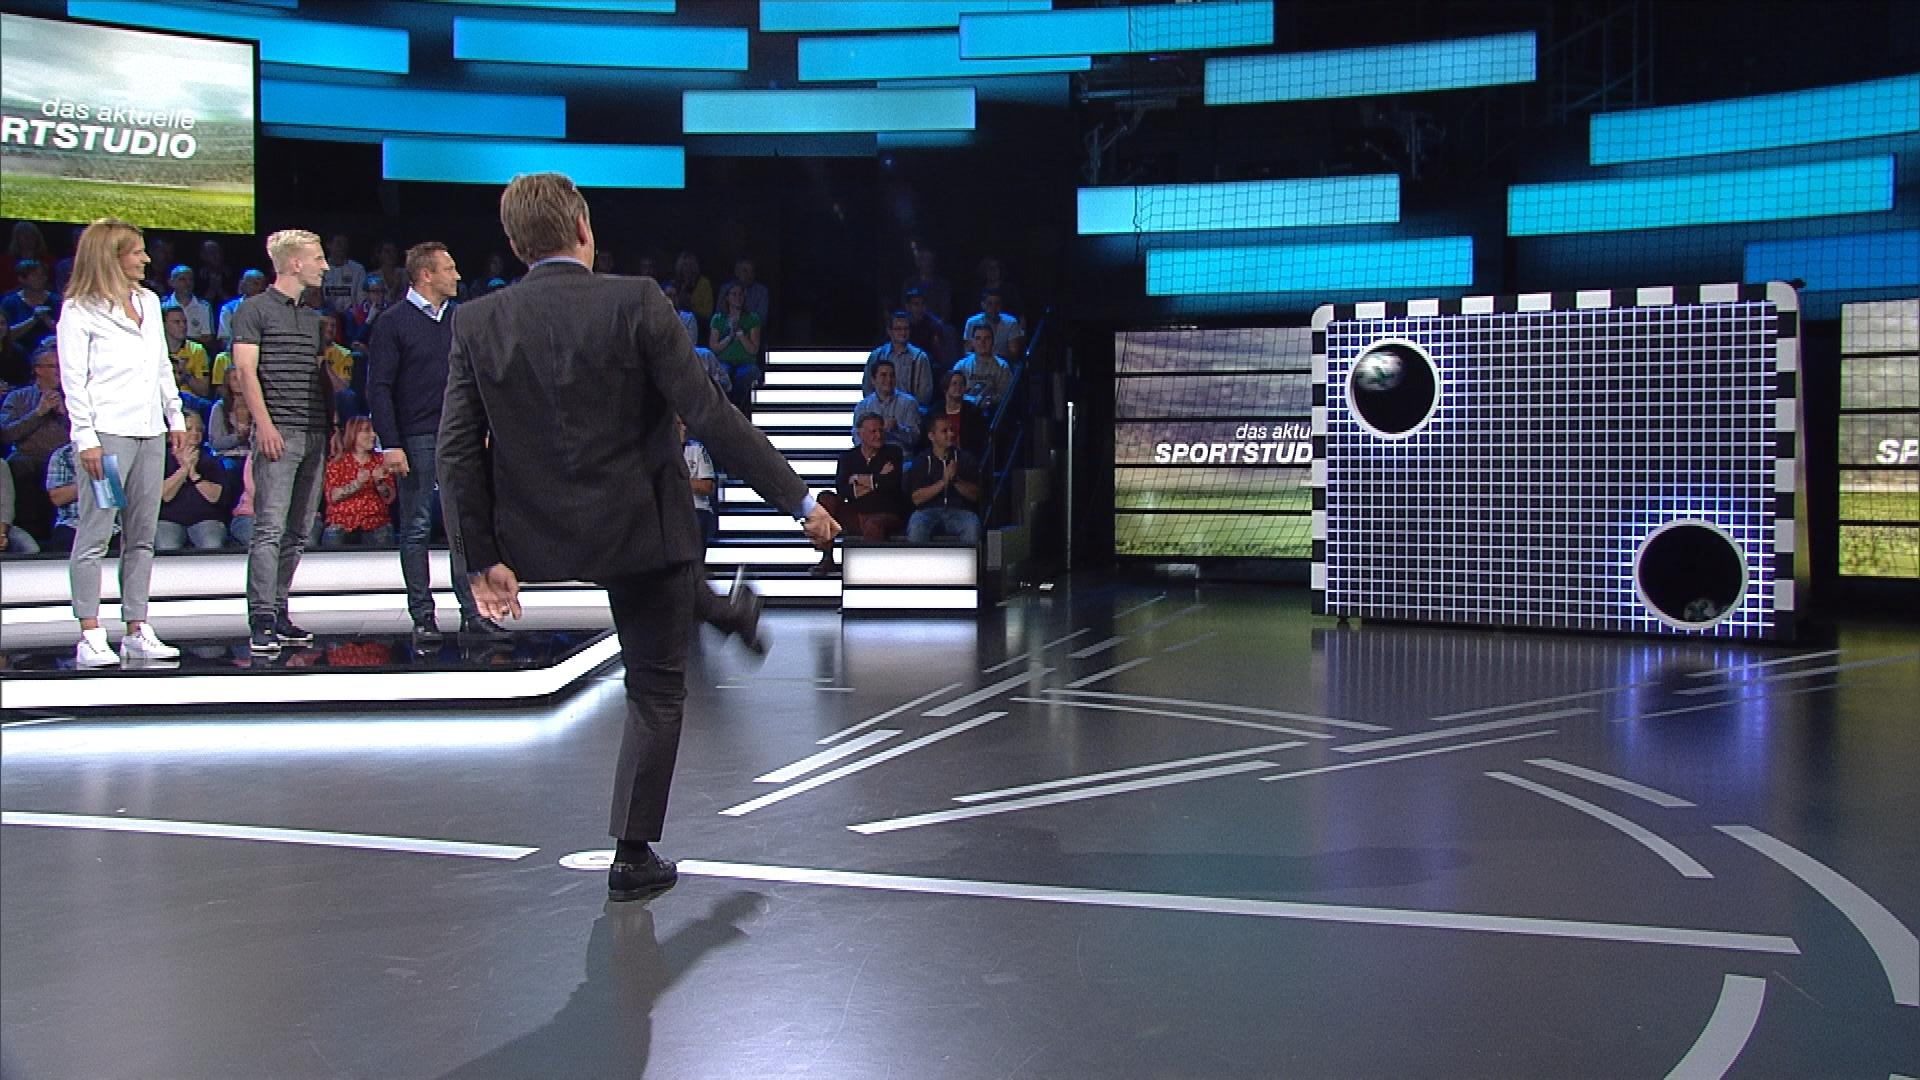
\includegraphics[width=0.7\linewidth]{torwandschiessen.jpeg}
	\caption{Torwandschißen}
	\label{fig:overview}
\end{figure}

\section{Requirements}
\begin{itemize}	
	\item Kinect Sensor
  \item Microsoft Hololens
\end{itemize}

\section{Weekly milestones}
\begin{itemize}	
  \item Body tracking using the Kinect sensor
  \item Mapping the body motion to a rigged 3d avatar in a normal Unity application
  \item Setting up the Holo-lens specific Unity application with the virtual elements
  \item Establishing a pipeline to transfer Kinect body motion data to the Unity application
  \item Use the Unity physics engine to project the ball onto the target
  \item Add visual feedbacks for the user and gamify the application
\end{itemize}


\section{Team}
\begin{itemize}
\item Marcel Bruckner
\item Kevin Bein
\item Jonas Schulz
\item Chandramohan Sudar
\end{itemize}


% references
{\small
	\bibliographystyle{plain}
	\bibliography{project_proposal}
}

\end{document}


